%% ----------------------------------------------------------------
%% Thesis.tex -- MAIN FILE (the one that you compile with LaTeX)
%% ---------------------------------------------------------------- 

% Set up the document
\documentclass[a4paper, 11pt, oneside]{uet_thesis}  % Use the "Thesis" style, based on the ECS Thesis style by Steve Gunn
\graphicspath{{Figures/}}  % Location of the graphics files (set up for graphics to be in PDF format)

% Include any extra LaTeX packages required
\usepackage[square, numbers, comma, sort&compress]{natbib}  % Use the "Natbib" style for the references in the Bibliography

\usepackage{verbatim}  % Needed for the "comment" environment to make LaTeX comments

\usepackage{vector}  % Allows "\bvec{}" and "\buvec{}" for "blackboard" style bold vectors in maths

\usepackage{url}
\usepackage{natbib}
\usepackage{amsmath}

\hypersetup{urlcolor=blue, colorlinks=true}  % Colours hyperlinks in blue, but this can be distracting if there are many links.

% remove the unnecessary spacing before and after the headings/subheadings
\usepackage[compact]{titlesec}
\titlespacing{\section}{0pt}{*0}{*0}
\titlespacing{\subsection}{0pt}{*0}{*0}
\titlespacing{\subsubsection}{0pt}{*0}{*0}

\setlength{\parskip}{6pt}
%\setlength{\parsep}{0pt}
%\setlength{\headsep}{0pt}
%\setlength{\topskip}{0pt}

%% ----------------------------------------------------------------
\begin{document}
	\frontmatter	  % Begin Roman style (i, ii, iii, iv...) page numbering
	
	% Set up the Title Page
	\title  {Gate Driver for N-Channel
		MOSFET}
	\session {2015 -- 2019}
	\advisor {Dr. Abdul Rehman Kashif}
	\authors {
		Hafiz Abubakar Azeem ~~~ 2015-EE-137 \\}
	
	\addresses  {\deptname \\ \univname}  % Do not change this here, instead these must be set in the "Thesis.cls" file, please look through it instead
	\date       {\today}
	\subject    {}
	\keywords   {}
	
	\maketitle
	%% ----------------------------------------------------------------
	\centering
	\section{4N35}
	
	\begin{figure}[htbp]
	\centering
	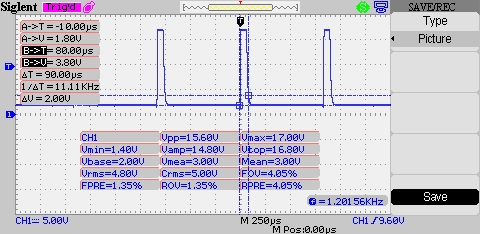
\includegraphics[width = 2.8in]{./Figures/4n35/1}
\end{figure}	

	\begin{figure}[htbp]
	\centering
	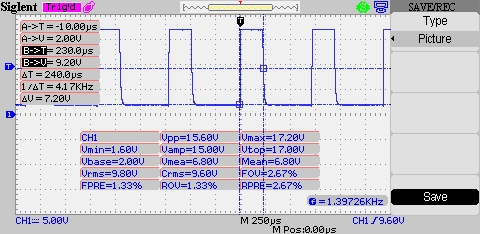
\includegraphics[width = 2.8in]{./Figures/4n35/3}
\end{figure}	

	\begin{figure}[htbp]
	\centering
	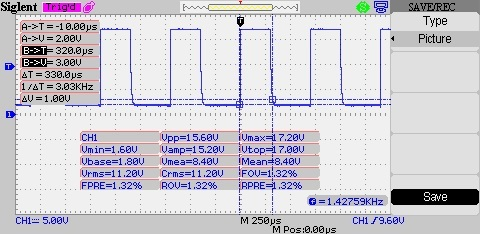
\includegraphics[width = 2.8in]{./Figures/4n35/5}
\end{figure}	

	\begin{figure}[htbp]
	\centering
	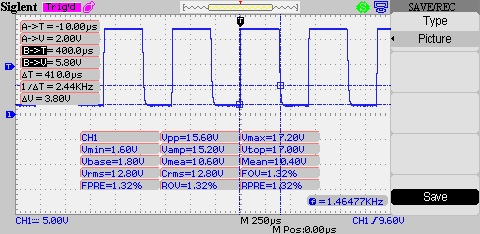
\includegraphics[width = 2.8in]{./Figures/4n35/7}
\end{figure}	

	\begin{figure}[htbp]
	\centering
	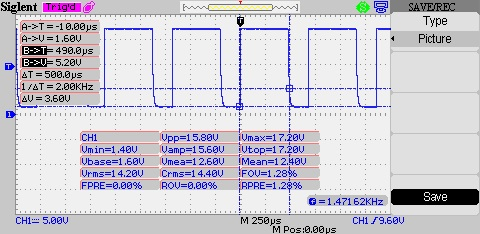
\includegraphics[width = 2.8in]{./Figures/4n35/9}
\end{figure}	
	\newpage
\section{TLP250}

\begin{figure}[htbp]
	\centering
	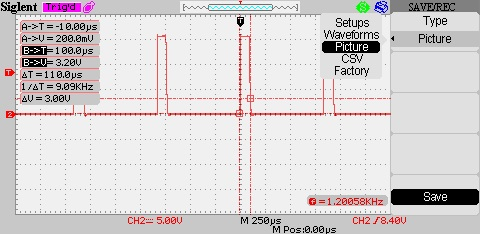
\includegraphics[width = 2.8in]{./Figures/tlp/1}
\end{figure}	

\begin{figure}[htbp]
	\centering
	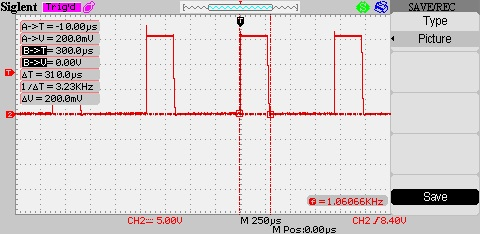
\includegraphics[width = 2.8in]{./Figures/tlp/2}
\end{figure}	

\begin{figure}[htbp]
	\centering
	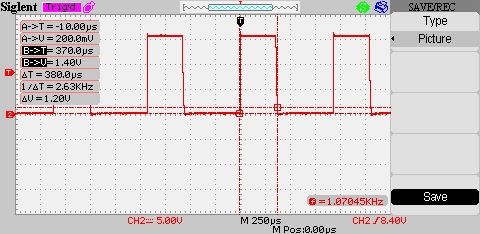
\includegraphics[width = 2.8in]{./Figures/tlp/3}
\end{figure}	

\begin{figure}[htbp]
	\centering
	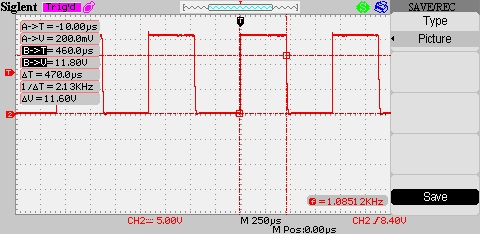
\includegraphics[width = 2.8in]{./Figures/tlp/4}
\end{figure}	

\begin{figure}[htbp]
	\centering
	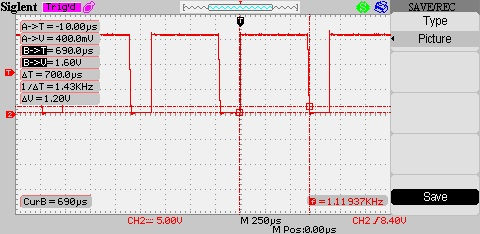
\includegraphics[width = 2.8in]{./Figures/tlp/5}
\end{figure}	

\newpage
\section{IRF2103}

\begin{figure}[htbp]
	\centering
	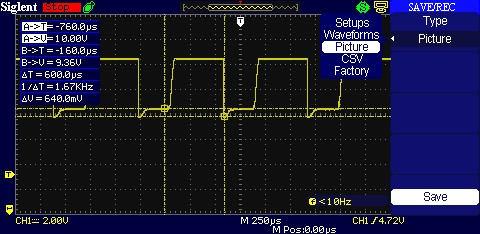
\includegraphics[width = 2.8in]{./Figures/irf/1}
\end{figure}	

\begin{figure}[htbp]
	\centering
	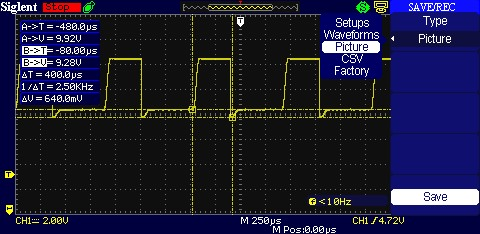
\includegraphics[width = 2.8in]{./Figures/irf/2}
\end{figure}	

\begin{figure}[htbp]
	\centering
	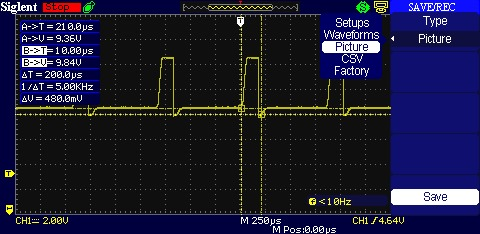
\includegraphics[width = 2.8in]{./Figures/irf/3}
\end{figure}	



\end{document}  % The End
%% ----------------------------------------------------------------
